\documentclass{standalone}
\usepackage{tikz}


\renewcommand\familydefault\sfdefault
\usetikzlibrary{positioning,calendar}

\def\generalcolor{green!50!black}
\def\currentyear{2023}
\def\s{0.9}
\def\colsep{20}
\def\colsepmonth{20}

\newcommand{\calrow}[1]{
  \node[\generalcolor, anchor=east,scale=\s](Mon) at(0,0){Mon};
  \node[\generalcolor, anchor=east,scale=\s](Tue) at(\colsep pt,0){Tue};
  \node[\generalcolor, anchor=east,scale=\s](Wed) at(2*\colsep pt,0){Wed};
  \node[\generalcolor, anchor=east,scale=\s](Thu) at(3*\colsep pt,0){Thu}; 
  \node[\generalcolor, anchor=east,scale=\s](Fri) at(4*\colsep pt,0){Fri};
  \node[\generalcolor, anchor=east,scale=\s](Sat) at(5*\colsep pt,0){Sat};
  \node[\generalcolor, anchor=east,scale=\s](Sun) at(6*\colsep pt,0){Sun};
  \node[\generalcolor, anchor=center, yshift=\colsep pt] at(Thu) {\bfseries\MakeUppercase{#1}};
}

\newcommand{\calperiod}[2][\currentyear]{%
  \calendar[dates=\currentyear-#2-01 to \currentyear-#2-last]
    if (Saturday, Sunday) [\generalcolor] \holidays;}

\newcommand{\holidays}{% holidays in Italy
% if (equals=01-01) [holiday]%
% if (equals=01-06) [holiday]%
% if (equals=04-04) [holiday]%
% if (equals=04-05) [holiday]%
% if (equals=04-25) [holiday]%
% if (equals=05-01) [holiday]%
% if (equals=05-01) [holiday]%
% if (equals=06-02) [holiday]%
% if (equals=08-15) [holiday]%
% if (equals=11-01) [holiday]%
% if (equals=12-08) [holiday]%
% if (equals=12-25) [holiday]%
% if (equals=12-26) [holiday]%
}
\begin{document}
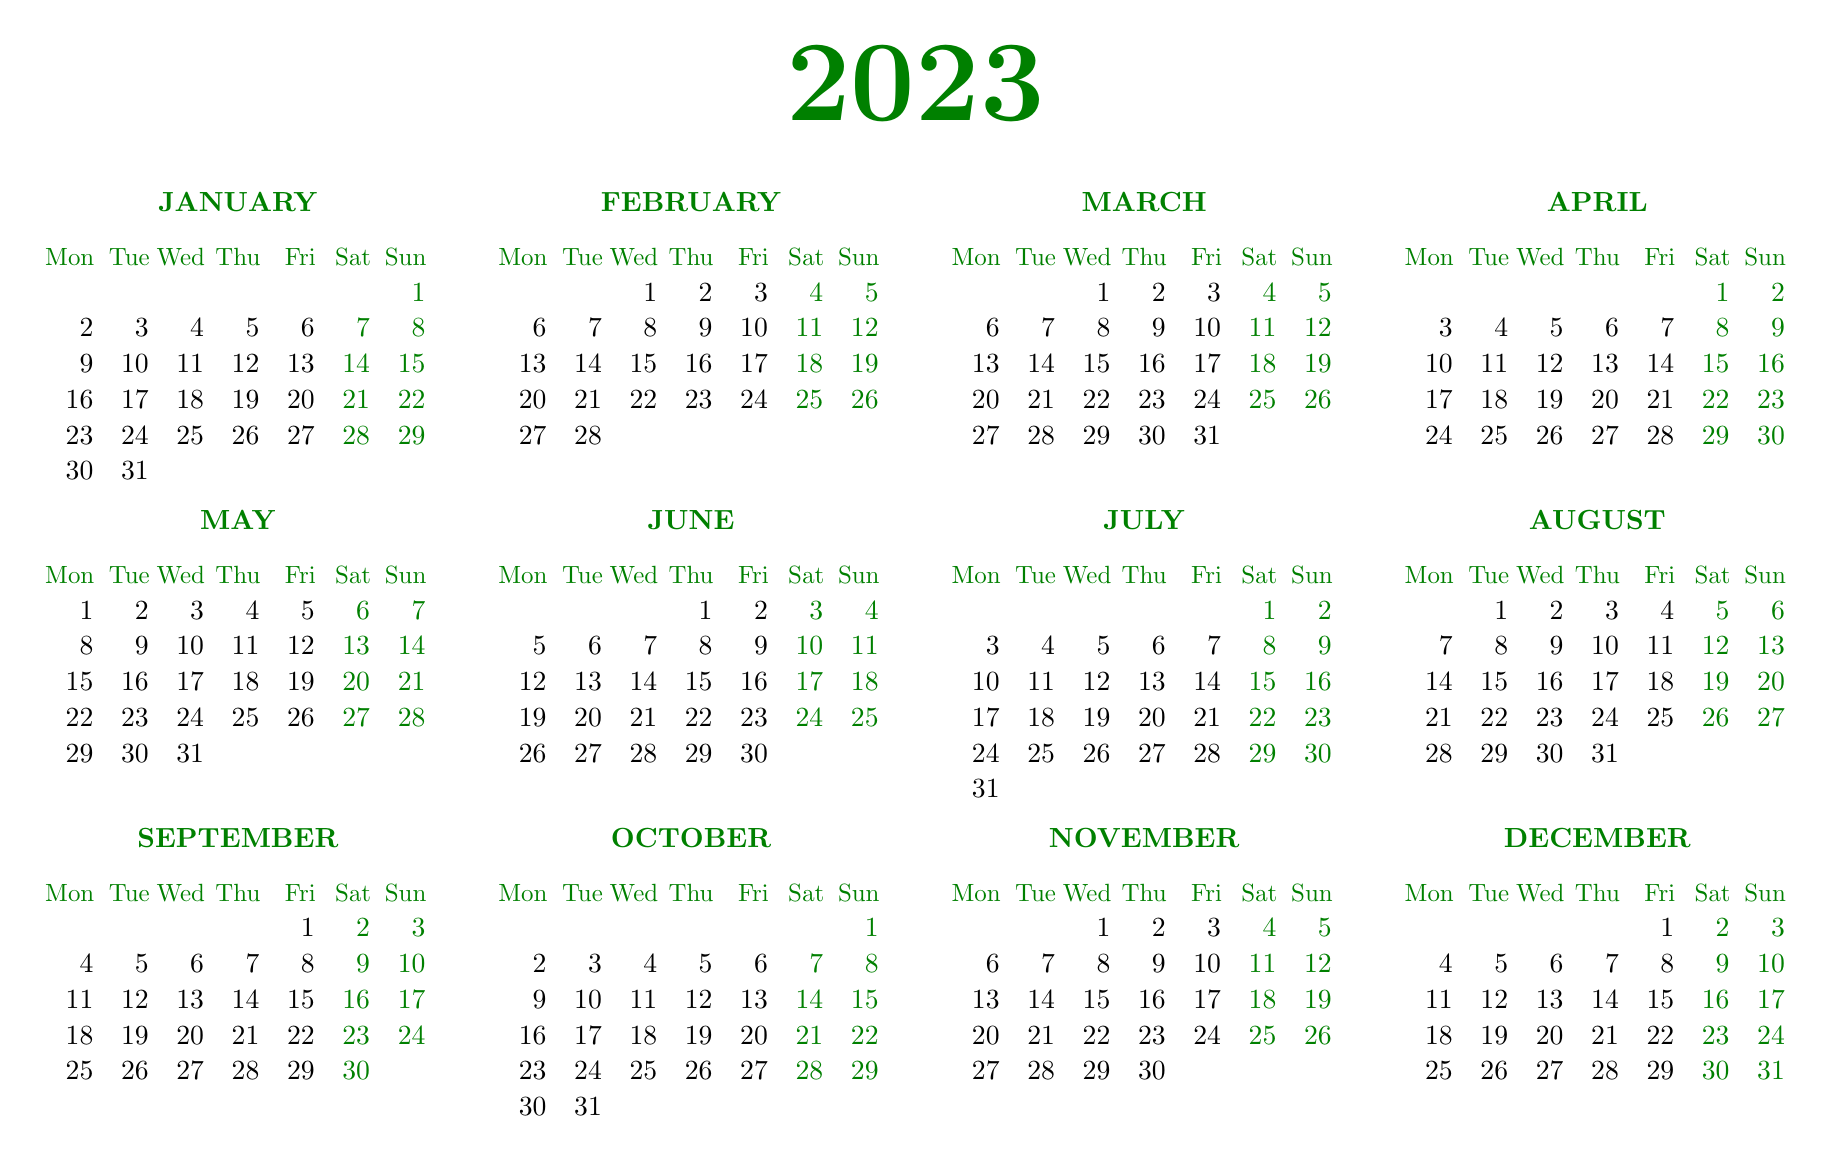
\begin{tikzpicture}[every calendar/.style={
        week list,
        day xshift=20pt,
      },
    year label/.style={
        fill=white,
        text=\generalcolor,
        font=\bfseries\Large
      }]
  \node[text=\generalcolor, font=\huge, scale=2] at (0,7.25){\bfseries\currentyear};
  \matrix[%
    column sep=\colsepmonth pt,%
    % draw=\generalcolor,thick,rounded corners=5pt,%
  ]{%

    % first row: week day and month
    \calrow{January}   & \calrow{February} & \calrow{March}    & \calrow{April}    \\
    \calperiod{01}     & \calperiod{02}    & \calperiod{03}    & \calperiod{04}    \\[1ex]

    % second row: calendar
    \calrow{May}       & \calrow{June}     & \calrow{July}     & \calrow{August}   \\
    \calperiod{05}     & \calperiod{06}    & \calperiod{07}    & \calperiod{08}    \\[1ex]

    % third row: week day and month
    \calrow{September} & \calrow{October}  & \calrow{November} & \calrow{December} \\
    \calperiod{09}     & \calperiod{10}    & \calperiod{11}    & \calperiod{12}    \\[1ex]
  };

\end{tikzpicture}
\end{document}